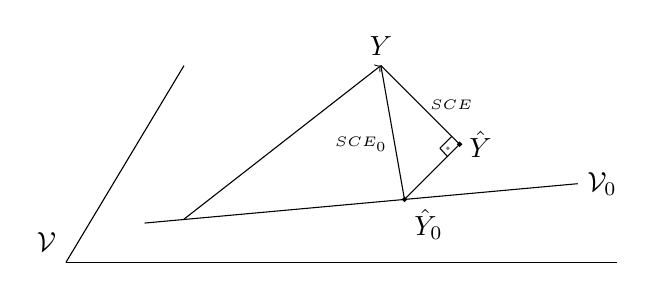
\begin{tikzpicture}
	% EV V
	\draw (0,-0.5) -- (1.5,2);
	\draw (0,-0.5) -- (7,-0.5);
	\node [below left] at (0,0) {$\mathcal{V}$};
	% V_0
	\draw (1, 0) -- (6.5, 0.5);
	\node [right] at (6.5, 0.5) {$\mathcal{V}_0$};
	% Y
	\draw[->] (1.5, 0.05) -- (4, 2);
	\node[above] at (4, 2) {$Y$};
	% \hat{Y}_0
	\draw (4.3, 0.3) -- (4, 2);
	\draw[fill] (4.3, 0.3) circle [radius=0.025]; 
	\node[below right] at (4.3, 0.3) {$\hat{Y}_0$};
	% \hat{Y}
	\draw (5, 1) -- (4, 2);
	\draw[fill] (5, 1) circle [radius=0.025]; 
	\node[right] at (5, 1) {$\hat{Y}$};
	% SCE_0
	\node[left] at (4.2, 1) {\tiny $SCE_0$};
	% SCE
	\node[right] at (4.5, 1.5) {\tiny $SCE$};
	% Incremento variabilidad
	\draw (5, 1) -- (4.3, 0.3);
	% Angulo recto
	\draw (4.9, 1.1) -- (4.75, 0.95);
	\draw (4.85, 0.84) -- (4.75, 0.95);
	\draw[fill, gray] (4.85, 0.95) circle [radius=0.015]; 
\end{tikzpicture}